\documentclass[11pt]{exam}
\usepackage{style/preamble}
\newcommand{\name}{Section 6: Regression Discontinuity Design}


\begin{document}
\noindent
\fbox{%
  \begin{minipage}[t]{\linewidth}
    \class, \term \hfill
    \begin{center}
      \textbf{\Large \name}
    \end{center}
    \emph{\tanames} \hfill
  \end{minipage}
}
\begingroup\small

\section{Observational Studies}
So far our discussions have been limited to randomized experiments. That is, we randomized the treatment with a known assignment mechanism and used our knowledge of the assignment mechanisms to draw conclusions of the causal effect. However, often we do not have access to data from randomized experiments. Experiments are not only expensive, but can also be unethical. For example, when studying the effect of alcohol on mortality rates, we cannot force people to start drinking. 

Thus, we have to content with \emph{observational} data, i.e., data that has been collected, where the treatment has not been randomly assigned or we are unaware of the assignment mechanism. Think about studying the effect of a welfare program on a population or the effect of college on long-term earning. In the next part of the course, we study how we can identify the causal effect of questions like these.

\subsection{Assumptions in Observation Studies}
Lets recall our notation. Let $T$ be the treatment and $Y$ be the outcome of interest. Typically, we assume that $T \in \{0, 1\}$ but we do not impose the same on $Y$. We also observe pre-treatment covariates $X$ (age, gender, \ldots). Unless otherwise stated, we assume i.i.d. sampling, i.e.,
\[
    \{X_i, T_i, Y_i(0), Y_i(1)\}_{i=1}^n \iid \mathbb{P}^\ast,
\]
from an unknown super-population. Throughout this part of the course, we make the following assumptions.
\begin{assumption}[SUTVA]\label{ass:sutva}
We have 
\begin{enumerate}
    \item \emph{No interference:} $Y_i(T_1,\dots,T_n)=Y_i(T_i)$; treatments on other units do not affect unit $i$
    \item \emph{Consistency:} $Y_i = Y_i(T_i)$; the observed outcome equals the corresponding potential outcome.
\end{enumerate}
\end{assumption}

\begin{assumption}[Strong Ignorability/Unconfoundedness]\label{ass:strong_ignorability}
    We have
    \[
    \{Y(1), Y(0)\} \ind T \mid X.
    \]
\end{assumption}
% This means that, conditional on the observed covariates $X$, treatment assignment is as good as random. In other words, there are no unobserved confounders that jointly affect both $T$ and $Y$. \textcolor{blue}{add explanation here with an example. refer to tablets in school, make DAG of acceptable and not acceptable ignorability assumption.}

\begin{assumption}[Strong Overlap]\label{ass:strong_overlap}
    There exists $\eta \in (0, \frac{1}{2})$ such that
    \[
    \eta < \Pr(T = 1 \mid X) \leq 1 - \eta.
    \]
    \noindent 
\end{assumption}
Strong overlap ensures that for all values of $X$, every unit has a positive probability of receiving either treatment. Without overlap, it becomes impossible to compare treated and untreated units with similar covariates (lack of observed counterfactuals). Often, we abbreviate $e(x) = \Pr(T = 1\mid X = x)$, which is called the \emph{propensity score}.

We have already seen SUTVA before, but what about Assumptions~\ref{ass:strong_ignorability} and~\ref{ass:strong_overlap}? To understand assumptions, its always a good idea to investigate when they fail. Assume a physician gives treatments to a patient, then our assumptions might be violated
\begin{itemize}
    \item Strong Ignorability: If a physician assigns a treatment based on an unrecorded severity score that also influences recovery, then $T$ and $Y$ are not independent given $X$.
    \item Strong Overlap: If all young patients are always treated and all older patients are never treated, then we cannot identify treatment effects for either group.
\end{itemize}

Both, strong ignorability and strong overlap are generally untestable assumptions. However, while strong ignorability often must be qualitatively argued (although we see we see a quantitative approach later on via negative controls), strong overlap can be much easier ``verified" when looking directly at the data (e.g., by plotting a histogram of the propensity score and see whether it falls within $[\eta, 1 - \eta]$ for some $\eta > 0$ and does not seem to converge to the boundary). Especially if our covariates are discrete, we could just check every covariate combination (if we had enough data).


\subsection{Tension between Ignorability and Overlap}
In observational studies, causal inference fundamentally relies on two key assumptions: \emph{ignorability} and \emph{overlap}. 
As emphasized by \citet{d2021overlap}, these two assumptions are often in tension. 
Including more covariates typically makes the ignorability assumption more plausible, since it becomes less likely that important confounders are omitted. But at the same time more covariates make the overlap assumption less plausible, as the treatment assignment tends to become more predictable. Thus the propensity score will be closer to $0$ or $1$, which will make our methods numerically unstable. Consequently, it is important to find the right balance of how many covariates to include.

\subsection{Assessing Ignorability Using Negative Controls}
This subsection follows the excellent notes of \citet[Sections~16.2.1--16.2.2]{ding2023coursecausalinference}. 
Since ignorability is fundamentally untestable, we can only assess its plausibility through supplementary analyses. Two common strategies rely on \emph{negative outcomes} and \emph{negative exposures}, which provide indirect evidence that adjusting for $X$ removes confounding.

\subsubsection{Negative Outcomes}\label{sec:negative_outcomes}
Suppose $Y^{n}$ is an outcome that shares the same confounding structure as the main outcome $Y$ but is known, by design, to be unaffected by the treatment $T$. If we believe that $\{Y(1), Y(0)\} \ind T \mid X$ this might imply that $ \{Y^n(1), Y^n(0)\} \ind T \mid X$. If the latter is true, then
\begin{align*}
    0 &=\E[Y^n(1) - Y^n(0)] 
    \\
    &=\E[ \E[Y^n(1) - Y^n(0) \mid X]]
    \\
    &= \E[\E[Y^n \mid T = 1, X]] - \E[\E[Y^n \mid T = 0, X]].
\end{align*}
We can estimate the last expression. When the effect is very different from zero, this suggests residual confounding. However, if we do not reject, this does not mean that ignorability holds. 

A causal diagram illustrating this logic is shown below:
\[
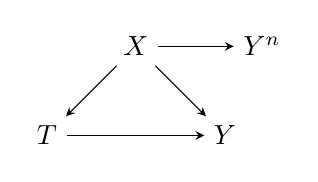
\begin{tikzpicture}[>=stealth, node distance=1.6cm]
  \node (X) {$X$};
  \node[right of=X] (Yn) {$Y^n$};
  \node[below right of=X] (Y) {$Y$};
  \node[below left of=X] (T) {$T$};
  \draw[->] (X) -- (T);
  \draw[->] (X) -- (Y);
  \draw[->] (X) -- (Yn);
  \draw[->] (T) -- (Y);
\end{tikzpicture}
\]
\noindent
\paragraph{Example:} \citet{cornfield1959smoking} studied smoking and lung cancer, and used car accidents as a negative outcome. The effect of smoking on accidents was near zero, consistent with randomization.
Similarly, \citet{jackson2006evidence} examined influenza vaccination and mortality. The observed reduction in mortality before flu season (when vaccines cannot yet act) indicated unmeasured confounding.

\subsubsection{Negative Exposures}
Negative exposures reverse the logic. 
Suppose $T^{n}$ is a placebo treatment that shares the same confounding structure as $T$, but is known not to causally affect $Y$. If we believe that $\{Y(1), Y(0)\} \ind T \mid X$ this might imply that $ \{Y(1), Y(0)\} \ind T^n \mid X$. In this case, we have
\begin{align*}
    0 &=\E[Y(1^n) - Y(0^n)] 
    \\
    &=\E[ \E[Y(1^n) - Y(0^n) \mid X]]
    \\
    &= \E[\E[Y \mid T^n = 1, X]] - \E[\E[Y \mid T^n = 0, X]].
\end{align*}
Then observing a nonzero association between $T^{n}$ and $Y$ given $X$ signals unmeasured confounding.
A representative causal diagram is:
\[
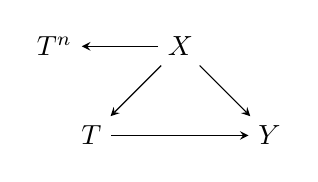
\begin{tikzpicture}[>=stealth, node distance=1.6cm]
  \node (X) {$X$};
  \node[below right of=X] (Y) {$Y$};
  \node[below left of=X] (T) {$T$};
   \node[left of=X] (Tn) {$T^n$};
  \draw[->] (X) -- (T);
  \draw[->] (X) -- (Y);
  \draw[->] (X) -- (Tn);
  \draw[->] (T) -- (Y);
\end{tikzpicture}
\]
\noindent
\paragraph{Example:}\citet{sanderson2018negative} proposed using paternal smoking as a negative exposure when estimating the effect of maternal smoking on autism of their offspring. If both maternal and paternal smoking share similar confounding, a larger effect for the mother than for the father supports a causal mechanism.

\subsection{Implications of Strong Overlap}
This subsection is motivated by the excellent notes of \citet[Section~20.1]{ding2023coursecausalinference}, which are based on \citet{d2021overlap}.
It turns out that Assumption~\ref{ass:strong_overlap} of strong overlap has quite strong implications on our covariates. Assume that $X \in \R^p$ and let
\begin{align*}
    P_0(X) &= P_0(X \mid T = 0)
    \\
    P_1(X) &= P_1(X \mid T = 1)
\end{align*}
be the probability measures of the covariates under control and treatment. Define $\Sigma_0 = \Var_{P_0}(X)$ and $\Sigma_1 = \Var_{P_1}(X)$ as the covariances matrices of $X$ under $P_0$ and $P_1$. Further, let $e = \Pr(T=1)$.

\begin{theorem}[\citet{d2021overlap}, Corollary 1]
Assumption~\ref{ass:strong_overlap} implies
   \[
   \frac{1}{p} \sum_{k=1}^p |\E[X_k \mid T = 1] - \E[X_k \mid T = 0]| \leq \frac{1}{\sqrt{p}} \min \left \{C_1(e, \eta)  \sqrt{ \|\Sigma_1 \|_{\text{op}}}, C_0(e, \eta)  \sqrt{\|\Sigma_0 \|_{\text{op}}} \right\},
   \]
   where $C_1(e, \eta), C_0(e, \eta)$ are constants depending on $e$ and $\eta$ and $\|.\|_{\text{op}}$ denotes the operator norm (largest singular value of the matrix).
\end{theorem}
The left-hand site measures the absolute mean differences between covariates under treatment and control. The result implies that when $p \to \infty$ that unless the singular values of the covariances grow like $p$, the left-hand site vanishes. However, we can only have growing singular values if the variance must concentrate in a low-dimensional subspace under both groups. This means covariates must be highly collinear.
Hence, in high-dimensions strict overlap either forces near-mean-balance (on average) between covariates in treatment and control (i.e., does not allow for much difference in the groups) or a highly collinear covariance structure (think about what this implies for linear regression).

This motivates to consider identification strategies that work without Assumption~\ref{ass:strong_overlap}. One simple option is to trim units based on the estimated propensity score. Trimming then drops units within regions of little overlap. However, this changes the population and estimand. Another option is regression discontinuity desigm, which we will investigate in the next section.

\section{Regression Discontinuity Design}
Key for Regression discontinuity design (RDD) is the knowledge of the treatment assignment mechanism. There are two popular methods
\begin{enumerate}
    \item Sharp RDD: Treatment assignment is based on a deterministic rule,
    \item Fuzzy RDD: Encouragement to receive treatment is based on a deterministic rule.
\end{enumerate}
We will discuss both in turn. 
\section{Sharp RDD}
This section is heavily drawn from \citet[Section~20.2]{ding2023coursecausalinference} and \citet[Module~6]{chazal2024causalcoursenotes}.
Lets start with an example. Suppose you want to determine the effect of alcohol on motor vehicle accidents (mva). The drinking age in the US is 21, so those just under 21 years don't drink (in theory at least) and those above do drink. If alcohol then has an effect on mva, we should see an increase of mva at 21. This is in fact what we do observe, see Figure~\ref{fig:rdd_drinking_age}. However, can we attribute this spike to a causal relationship?

\begin{figure}
    \centering
    
\includegraphics[width=0.8\linewidth]{figures/rdd_drinking_age (1).pdf}
    \caption{Minimum legal drinking age example; from \citet{carpenter2009effect}.}
    \label{fig:rdd_drinking_age}
\end{figure}

\subsection{Theory}
The idea of sharp RDD is to find a covariate $X$ such that the treatment assignment is deterministic
\[
    T = \indicator{X \geq c},
\]
for a threshold $c$. In our example, $T$ indicates the legal access to alcohol, $X$ is age and $c = 21$. Interestingly, this immediately implies Assumption~\ref{ass:strong_ignorability}
\[
    \{Y(1), Y(0)\} \ind T \mid X,
\]
as conditioning on $X$, $T$ is now a constant, which is always independent to random variables.
However, $T = \indicator{X \geq c}$, clearly violates Assumption~\ref{ass:strong_overlap} of strong overlap. By definition, we have
\[
  e(X) = \Pr(T=1 \mid X)
       = \indicator{X \ge c}
       = \begin{cases}
            1, & \text{if } X \ge c,\\
            0, & \text{if } X < c.
         \end{cases}
\]
Thus, our units who receive the treatment are fundamentally different to those who do not receive it, making a comparison difficult. However, the treatment status changes at the threshold $c$. Maybe, we have reason to believe that units just below and just above the threshold are not so different and that the only difference between the two is the treatment. This motivates to consider the average treatment effect at the cutoff point
\[
    \tau(c) = \E[Y(1) - Y(0) \mid X = c].
\]
What kind of assumptions do we need to identify this effect?
\begin{assumption}[Continuity] \label{ass:continuity}
In a neighborhood around the cutoff $c$,
\[
 \mu_t(x) = \E[Y(t) \mid X = x]
\]
is continuous for $t \in \{0, 1\}$.
\end{assumption}
\textcolor{blue}{bring example what it means, I think I have thw wrong interpreation - check out Kosuke's paper}
Assumption~\ref{ass:continuity} justifies to extrapolate from the control to treatment (and vice versa) around the threshold. This requires that nothing else is going on around the cutoff $X = c$ that could have caused the jump, even without the treatment. In particular, there should be no other shock, besides the treatment assignment. 

\begin{theorem}\label{thm:sharp_rdd_identification}
    Assume that $T = \indicator{X \geq c}$ and that Assumption~\ref{ass:continuity} holds. Then the local average treatment effect is identified at $X = c$ by
    \[
    \tau(c) = \lim_{x \downarrow c} \E[Y \mid X = x] - \lim_{x \uparrow c} \E[Y \mid X = x].
    \]
\end{theorem}

\begin{proof}
    Focusing on the potential outcome under treatment we have under continuity and consistency,
    \begin{align*}
        \E[Y(1) \mid X = c] &=  \lim_{x \downarrow c} \E[Y(1) \mid X = x] = \lim_{x \downarrow c} \E[Y \mid X = x].
    \end{align*}
    Similarly, under control we have 
    \[
    \E[Y(0) \mid X = c] = \lim_{x \uparrow c} \E[Y \mid X = x],
    \]
    which together yield the desired result.
\end{proof}
Theorem~\ref{thm:sharp_rdd_identification} highlights that the estimand of interest is only valid locally around the threshold. Effects might differ quite substantially outside a neighborhood outside it. This is one of the key disadvantages of RDD, it is only internally, but not externally valid.

\subsection{Estimation}
Let $\tilde X = X - c$ such that $\tilde X \geq 0$ if and only if $X \geq c$.  
\subsubsection{Linear Regression}
If we pose $\mu_t(\tilde x) = \E[Y(t) \mid \tilde X = \tilde x]= \alpha_t + \beta_t \tilde x$ then we could simply fit two linear regressions or, simpler (but equivalent), one regression with full interactions
\[
    Y_i = \alpha_i + \beta \tilde X_i + \tau T_i + \gamma \tilde X_i T_i.
\]
This fits $\hat \mu_0(\tilde x) = \hat \alpha + \hat \beta \tilde x$ and $\hat \mu_1(\tilde x) = (\hat \alpha + \hat \tau) + (\hat \beta + \hat \gamma) \tilde x$. Our estimate by Theorem~\ref{thm:sharp_rdd_identification} is then obtained by
\begin{align*}
    \hat \tau(c) &=  \lim_{x \downarrow c} \widehat{\E[Y \mid X = x]} - \lim_{x \uparrow c} \widehat{\E[Y \mid X = x]}
    \\
    &= \lim_{\tilde x \downarrow 0} \widehat{\E[Y \mid \tilde X = \tilde x]} - \lim_{\tilde x \uparrow 0} \widehat{\E[Y \mid \tilde X = \tilde x]}
    \\
    &= \hat \mu_1(0) - \hat \mu_0(0)
    \\
    &= (\hat \alpha + \hat \tau) - \hat \alpha
    \\
    &= \hat \tau.
\end{align*}
Essentially, we are fitting one linear regression above and another one below the threshold. The full interaction approach has the advantage of only needing to run one regression once. We can then use a heteroskedasticity-robust estimator to estimate $\widehat{\Var}(\hat \tau(c))$, as we have seen in the linear regression chapter.

The linear regression approach is quite simple. However, we not only assume linearity, but we use all observations, no matter how far they are away from the threshold. If we have only few observations near the threshold, that might severely bias the analysis.

\subsubsection{Polynomial Regression}
To add more flexibility to the model, we could alternatively pose a polynomial regression
\[
    \mu_t(\tilde x) = \E[Y(t) \mid \tilde X = \tilde x] = \alpha_t + \beta_{t1}\Tilde{X} +  \beta_{t2}\Tilde{X}^2 + \ldots  + \beta_{tk}\Tilde{X}^k,
\]
and again fit a fully interacted model to obtain our estimates. However, \citet{gelman2019high} have argued that this is a bad idea as it leads to noisy estimates, is sensitive to the degree of the polynomial, and has poor coverage of confidence intervals. Thus, it is not recommended to run polynomial regression with degrees $k \geq 3$.

\subsubsection{Local Linear Regression}
The main issue with linear regression is that it includes all observations, no matter their distance from the cutoff point. Local linear regression exactly addresses this. Instead of fitting (two) linear regressions on all data points, we fit them only around the cutoff
\[
    \hat \alpha, \hat \beta, \hat \tau, \hat \gamma = \argmin_{\alpha, \beta, \tau, \gamma} \sum_{i=1}^n (Y_i - \alpha - \beta \tilde X_i - \tau T_i - \gamma \tilde X_i T_i)^2 K\left(\frac{\tilde X_i}{h}\right),
\]
for a pre-specified bandwidth $h$ and kernel function $K$. 
Typically, we use the window kernels $K(x) = \indicator{|x| \leq 1}$ or triangular kernel $K(x) = \max\{0, 1 - |x|\}$. The window kernel then only counts observations within the window $[c-h, c + h]$, while the triangular kernel does the same, but weights observations more the closer they are to the cutoff. Essentially this is just \emph{weighted} linear regression with weights $w_i = K\left(\frac{\tilde X_i}{h}\right)$. Note that we could have also included polynomial terms (up to second degree) in the regression. Our estimator is again given by 
\[
    \hat \tau(c) = \hat \tau,
\]
and we can again use a heteroskedasticity-robust estimator to estimate its variance. The question remains on how to choose the bandwidth $h$. One principled way of doing it, proposed by \citet{imbens2012optimal}, is to choose $h$ to minimize the bias-variance trade-off. If $h$ is large, we might include observations far from the cutoff, making our estimates biased. If $h$ is small, then we might have too few observations in our regression and our results become noisy. Thus we could minimize 
\begin{align*}
    \mathrm{MSE} = \E[(\hat \tau_h(c) - \tau (c))^2] = \mathrm{Bias}_h^2 + \mathrm{Variance}_h.
\end{align*}
Using local approximations, the $\texttt{R}$ package $\texttt{rdrobust}$ implements this with the function $\texttt{rdbwselect}$.

For local linear regression estimation, we even have the following theoretical guarantee.
\begin{theorem}[\citet{wagerathey2023causalinference}, Proposition~8.1]
    Suppose that $X$ has a continuous distribution around the cutoff $c$ and $\Var(Y_i \mid T_i = t) \leq \sigma^2$ for $t \in \{0, 1\}$. Suppose further that $\mu_t(x) = \E[Y(t) \mid X = x]$ is twice continuously differentiable and its second derivative is uniformly bounded for $t \in \{0, 1\}$ (this is stronger than Assumption~\ref{ass:continuity}). Then the local linear regression estimator with bandwidth $h_n = \kappa n^{-1/5}$ for some $\kappa > 0$ is consistent and
    \[
        \hat \tau(c) = \tau(c) + \mathcal{O}(n^{-2/5}).
    \]
\end{theorem}

\subsubsection{Adding Covariates}
If we have further covariates $\bm{W}$ that we would like to include into the regression, we can simply add them to the local linear regression estimator
\[
    \hat \alpha, \hat \beta, \hat \tau, \hat \gamma, \bm{\hat{\delta}} = \argmin_{\alpha, \beta, \tau, \gamma} \sum_{i=1}^n (Y_i - \alpha - \beta \tilde X_i - \tau T_i - \gamma \tilde X_i T_i - \bm{\delta}^\top \bm{W})^2 K\left(\frac{\tilde X_i}{h}\right).
\]
We only require that the conditional distribution of $\bm{W}$ given $X$ is continuous at the cutoff $X = c$ \citep{imbens2008regression}.

\subsection{Diagnostics for Regression Discontinuity Design}
Our key assumption for RDD is that $\E[Y(t) \mid X = x]$ is continuous around a neighborhood of the cutoff $c$. When might this assumption fail? The two most common causes are \emph{competing shocks} and \emph{sorting/manipulation}. Competing shocks occur when at the threshold, other reasons might cause a jump in the outcome. Sorting occurs when the treatment assignment mechanism is known to individuals and they might sort themselves into the more favorable group. For example, one might report one's income just below the threshold to qualify for financial aid.
In the drinking-age example, violations can arise if:
\begin{itemize}
    \item \textbf{Competing Shocks}: 
    If another policy changes at age 21; e.g., access to other age-restricted activities that alter nighttime driving exposure.
    \item \textbf{Sorting/Manipulation}: If individuals use a fake driver's license (or borrow one from friends or family) that shows their age at 21 or above.
\end{itemize}

As with most assumptions in causal inference, we cannot directly test Assumption~\ref{ass:continuity}, but we can collect evidence for or reject consequences of it.

\subsubsection{Competing Shocks - Placebo Test}
\textcolor{blue}{tests whether other shocks affect the outcome, not the treatment (this is deterministic). Its the same as using negative outcomes.}
We try to verify whether competing shocks might have influenced the outcome outside of the treatment. We do this by checking that pre-treatment covariates that should not be affected by the treatment have continuous expected outcomes around the threshold. If they don't, this provides evidence that something else might be going on. How do we do that for a covariate $W$? Well, we can just to RDD on $W$!
\begin{enumerate}
    \item Plot $X$ vs. $W$ to visually inspect continuity at the threshold $c$
    \item Estimate $\tau_W(c)\;=\;\lim_{x \downarrow c}\E[W\mid X=x]\;-\;\lim_{x \uparrow c}\E[W\mid X=x]$ and test $\tau_W(c)=0$.
\end{enumerate}

Typical pre-treatment covariates include negative outcomes (see Section~\ref{sec:negative_outcomes}), which might be lagged outcomes from a previous time periods before the treatment was given. If we fail to reject the placebo test, this does not mean that our null is correct, just that we have more evidence for it.

\subsubsection{Sorting - McCrary Density Test}
\textcolor{blue}{test whether treatment is continuous distribution.}
Proposed by \citet{mccrary2008manipulation}. The idea is to test whether the density of the running variable $X$ is continuous at the cutoff $c$. Figure~\ref{fig:mccrary_density} illustrates when this fails.

\begin{figure}
    \centering
    
\includegraphics[width=0.8\linewidth]{figures/densitytest1.pdf}
    \caption{Percent voting yeay: roll call votes, U.S. House of Representatives, 1857–2004; from \citet{mccrary2008manipulation}.}
    \label{fig:mccrary_density}
\end{figure}


Let $f_X(c^-)$ and $f_X(c^+)$ denote the left- and right-hand limits of the density at $c$. The parameter of interest is the log jump $\psi \;=\; \log f_X(c^+) - \log f_X(c^-)$. Under no sorting/manipulation, $H_0:\ \psi=0$. A significant $\widehat{\psi}\neq 0$ indicates a discontinuity. For details on the inference, we refer to \citet{mccrary2008manipulation}. The estimation procedure is given by (again, refer to the paper for details)
\begin{enumerate}
    \item Construct a histogram of $X$
    \item Fit local linear regression to the midpoints to smooth the histogram
    \item Obtain $\widehat f_X(c^-)$ and $\widehat f_X(c^+)$ from around the threshold and estimate its difference
\end{enumerate}

The test is most informative when manipulation is \emph{monotone} (agents push $X$ in one direction). A continuous density is neither necessary nor sufficient for identification, so failing to reject $H_0$ does not prove validity alone.

\subsubsection{Local Randomization Not Required}\label{subsec:lr-not-required}
A common (but unnecessary) intuition for RD is that units just below and just above the cutoff are ``as-if randomly'' assigned to treatment in a small window. Formally, a local randomization assumption would posit some $h>0$ and the window $W(h)=\{i:\,|X_i-c|\le h\}$ such that,
\[
\{Y_i(0),Y_i(1)\}\ \ind\ T_i \mid i \in W(h)
\]
Local randomization implies $\mu_t(x)=\E[Y(t)\mid X=x]$ is flat over $[c-h,c+h]$ for $t\in\{0,1\}$, so a difference in means within $W(h)$ is justified. However, RDD identification does not require local randomization. We only assume continuity at the cutoff, which allows smooth trends (nonzero slopes) on either side. Assuming local randomization can actually be a disadvantage, when we do have different slopes around the cutoff, as illustrated in Figure~\ref{fig:rd}.

\begin{figure}
    \centering
    
\includegraphics[width=0.8\linewidth]{figures/RD.pdf}
    \caption{Figure from Kosuke Imais' Lecture Slides, Fall 2025}
    \label{fig:rd}
\end{figure}


\section{Fuzzy RDD}
This section is extended from \citet{chazal2024causalcoursenotes}.
In a sharp RDD design, we assume that the cut-off is deterministic. But in some real-world scenarios, it may be that actually, the cut-off is only an encouragement to get treatment as we discussed for instrumental variables in the previous chapter. For example, assume we want to study the effect of a receiving a high-school diploma on earnings. Receiving a diploma is highly non random, and thus traditional experimental methods won't work. An approach pursued by \citet{clark2014signaling} is to use test scores of high school exit exams as a running variable. The logic: students who just pass are not too different to students who just did not pass.  Passing can then be used as a cutoff for an RDD. If there is an effect, this would indicate that just the act of receiving the diploma (but not necessarily having learned more) would increase earning.

However, as it turns out, some students who did not pass, were still able to get a diploma (potentially through extra assignments etc.). Likewise, some students who did pass, also did not graduate. So the threshold is not deterministic, its acts more like an encouragement. This is exactly the type of setting we are studying with fuzzy RDD, which was first discussed by \citet{hahn2001identification}.

\subsection{Theory}
As with sharp RDD, define $Z = \indicator{X \geq c}$, as the encouragement or instrument variable. As with the IV setting, our potential outcomes are of the form $Y(z, T(z))$. We make the following assumptions, similar to the IV setting:
\begin{enumerate}
    \item \textbf{Monotonicity}: $T_i(1) \geq T_i(0)$. No defiers, i.e., no individuals will take the treatment only if not encouraged. In our example, people don't just receive a diploma \emph{because} they did not pass.
    \item \textbf{Exclusion}: $Y_i(z, t) = Y_i(t)$ for $z \in \{0, 1\}$. Only the diploma matters, not the test score.
    \item \textbf{Continuity}: $\E[T_i(z) \mid X_i = x$ and $\E[Y_i(z, T_i(z)) \mid X_i = x]$ are continuous in $x$ for $z \in \{0, 1\}$. This assumption replaces the randomization assumption from the IV setting.
    \item \textbf{Relevance}: $\lim_{x \downarrow c} \Pr(T_i = 1 \mid X_i = x) \neq \lim_{x \uparrow c}\Pr(T_i = 1 \mid X_i = x)$. Compare this to sharp RDD, where the jump between the probabilities is 1 \citep{imbens2008regression}.
\end{enumerate}
Under this assumptions, we can identify the (very) local average treatment effect on the compliers around the threshold,
\[
    \tau(c) = \E[Y_i(1) - Y_i(0) \mid T_i(1) > T_i(0), X_i = c] =
    \frac{\lim_{x \downarrow c} \E[Y \mid X = x] - \lim_{x \uparrow c} \E[Y \mid X = x]}{\lim_{x \downarrow c} \E[T \mid X = x] - \lim_{x \uparrow c} \E[T \mid X = x]}.
\]
This can be interpreted as the \emph{discontinuity} in $E[Y\mid X]$ over the \emph{discontinuity} in $E[T\mid X]$.
As with sharp RDD, the main issue with fuzzy RDD is that it lacks external validity. But now the problem is exacerbated, as we do not only condition on the threshold, but on compliers as well.

\subsection{Estimation}
As with sharp RDD, we can use local linear regression to estimate both the numerator and the denominator
\begin{align*}
    \hat \alpha_T, \hat \beta_T, \hat \tau_T, \hat \gamma_T &= \argmin_{\alpha, \beta, \tau, \gamma} \sum_{i=1}^n (T_i - \alpha - \beta \tilde X_i - \tau Z_i - \gamma \tilde X_i Z_i)^2K\left(\frac{\tilde X_i}{h}\right),
    \\
    \hat \alpha_Y, \hat \beta_Y, \hat \tau_Y, \hat \gamma_Y &= \argmin_{\alpha, \beta, \tau, \gamma} \sum_{i=1}^n (Y_i - \alpha - \beta \tilde X_i - \tau Z_i - \gamma \tilde X_i Z_i)^2 K\left(\frac{\tilde X_i}{h}\right),
\end{align*}
and set 
\[
    \hat \tau(c) = \frac{\hat \tau_Y}{\hat \tau_T}.
\]
Its variance can be estimated via bootstrap or the delta method. Alternatively, we can adapt also two-stage-least-square (2SLS) estimation.


\endgroup

\newpage

\bibliography{references}


\end{document}
